%!TEX root = main.tex

\chapter{Propositional Formulas and Models}

In this chapter, we start the discussion of propositional logic. We will define, how propositional formulas look, what is a model in propositional logic and we will also discuss some special forms of formulas.

Propositional logic is the more basic type of logic (and predicate logic is an extension of propositional logic in a sense).  Propositional formulas (propositions) are created from so called \emph{propositional variables} that represent an atomic fact which can either be true or false. These propositional variables can only be connected by common logic connectives ($\to$, $\lequiv$, $\land$, $\lor$, $\neg$). Logical formulas can additionally use parentheses to indicate the order of application of connectives. While the propositional formulas are simple compared to formulas in other types of logic, they are still useful. One of the most important problems in propositional logic and in computer science in general is the satisfiability of propositional formulas (SAT). Many other NP-complete problems are often solved by transformation to the SAT problem and using one of the existing SAT solvers.

\section{Syntax of Propositional Logic}

The set of propositional variables is often called $\Prop$ and the variables themselves are usually named $p, q, r, s$ or $p_0, p_1, \dots, q_0, q_1$, or similarly. Now, we can formally define the propositional formula (over $\Prop$).

\begin{definition}
Let $\Prop$ is the set of propositional variables, than
\begin{enumerate}
  \item Every propositional variable from $\Prop$ is a propositional formula.
  \item If $\varphi$ and $\psi$ are propositional formulas, than $(\varphi \to \psi), (\varphi \land \psi), (\varphi \lor \psi), (\varphi \lequiv \psi)$, and $(\neg \varphi)$ are propositional formulas.
  \item Every propositional formula is created by finite application of the two rules above.
\end{enumerate}
\end{definition}

The last part of the definition ensures that every formula is finite, this also means that each formula can contain only a finite number of distinct variables. The set of propositional variables used in a formula $\varphi$ will be denoted as $\Var(\varphi)$. On the other hand, the set of all propositional formulas using only variables from a set $\Prop$ will be denoted as $\VF_\Prop$.

Formulas are thus strings created from propositional variables, logical connectives, and parentheses, that fulfill the conditions in the definition above. A substring of such a string that also fulfills the conditions is called a \emph{sub-formula}. 

The formal definition of formula dictates the use of parentheses around every sub-formula, which can be rather cumbersome. Therefore, we define priorities of the logical connectives and can thus omit some of the parentheses. The standard priorities are such, that the negation ($\neg$) has the highest priority (therefore parentheses around $(\neg \varphi)$ can always be omitted), conjunction and disjunction ($\lor, \land$) have ``middle'' priority, and implication and equivalence ($\to, \lequiv$) have the lowest priority. Therefore, we can write $\varphi \land \psi \to \neg \varphi \lor \xi$ instead of $((\varphi \land \psi) \to ((\neg \varphi) \lor \xi))$. 

Each formula can be also represented by a so called \emph{formation tree}, which is a finite ordered tree, whose nodes are labeled with propositions -- the leaves are labeled with propositional variables, if a node has label $(\neg \varphi)$, it has a single son labeled with $\varphi$, and if a node has label $(\varphi \to \psi), (\varphi \land \psi), (\varphi \lor \psi),$ or $(\varphi \lequiv \psi)$, it has two sons, the left one has label $\varphi$, and the right one has label $\psi$. For example, a formula $p \land q \to \neg (p \lor s)$ is represented by the formation tree on the left.
\begin{marginfigure}[-4\baselineskip]
\centering
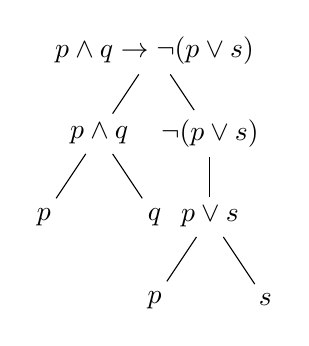
\begin{tikzpicture}[sibling distance=4em, level distance=3em]
  \node {$p \land q \to \neg (p \lor s)$}
    child { node {$p \land q$} 
      child {node {$p$}}
      child {node {$q$}} }
    child { node {$\neg (p \lor s)$}
    	child {node {$p \lor s$}
    		child {node {$p$}}
      	child {node {$s$}}}
     };
\end{tikzpicture}
\caption{The formation tree representing the formula $p \land q \to \neg (p \lor s)$.}
\end{marginfigure}

It is simple to show (by the induction on the number of nested parentheses) that each formula is associated with a unique formation tree. 

\section{Semantics of Propositional Logic}

Once we have the formal definition of the formula (the syntax of propositional logic), we can define its semantics (what the formula means). The propositional variables represent atomic statements, that can have one of two truth values -- either 0 (false) or 1 (true). The truth value of the whole proposition in then given by the truth values of the variables and by the semantics of the logical connectives, which is given in Table~\ref{tab:prop_semantics} bellow.

\begin{table}[h]
\centering
\caption{The semantics of logical connectives}
\label{tab:prop_semantics}
\begin{tabular}{cc|ccccc}
\toprule
$p$ & $q$ & $\neg p$ & $p \lor q$ & $p \land q$ & $p \to q$ & $p \lequiv q$ \\
\midrule
0 & 0 & 1 & 0 & 0 & 1 & 1 \\
0 & 1 & 1 & 1 & 0 & 1 & 0 \\
1 & 0 & 0 & 1 & 0 & 0 & 0 \\
1 & 1 & 0 & 1 & 1 & 1 & 1 \\
\bottomrule
\end{tabular}
\end{table}

We can also consider the table above a definition of Boolean functions $\lor_1, \land_1, \to_1, \lequiv_1,$ and $-_1$, that implement the logical connectives. We will use these functions in cases where it is needed (e.g. while talking about truth values of propositions). More generally, any propositional formula with $n$ variables defines a Boolean function $f: \{0,1\}^n \to \{0,1\}$ (later, we will also see that any Boolean function can be expressed using a propositional formula).

We also define two special logical formulas. The formula $\top \equiv p \lor \neg p$, which is always true, and the formula $\bot \equiv p \land \neg p$ which is always false.

We can now define the truth assignment and the truth value of formula more formally.

\begin{definition}
A \emph{truth assignment} is a function $v: \Prop \to \{0,1\}$, that is $v \in \fset{\Prop}{2}$.

A \emph{truth value} $\bar{v}(\varphi)$ of a propositional formula $\varphi$ for a truth assignment $v$ is defined inductively as:
	\begin{itemize}
		\begin{minipage}{0.5\textwidth}
		\item $\bar{v}(p) = v(p)$ if $p \in \Prop$
		\item $\bar{v}(\neg \varphi) = -_1(\bar{v}(\varphi))$ 
		\item $\bar{v}(\varphi \lor \psi) = \lor_1(\bar{v}(\varphi),\bar{v}(\psi))$ 
		\end{minipage}
		\begin{minipage}{0.5\textwidth}
		\item $\bar{v}(\varphi \land \psi) = \land_1(\bar{v}(\varphi),\bar{v}(\psi))$ 
		\item $\bar{v}(\varphi \to \psi) = \to_1(\bar{v}(\varphi),\bar{v}(\psi))$ 
		\item $\bar{v}(\varphi \lequiv \psi) = \lequiv_1(\bar{v}(\varphi),\bar{v}(\psi))$ 
		\end{minipage}
	\end{itemize}
\end{definition}

We can easily show (by the induction on the structure of the formula) that the truth value of a formula $\varphi$ depends only on the truth assignment of variables from $\Var(\varphi)$.

A proposition $\varphi$ over $\Prop$ is \emph{true in (satisfied by) an assignment} $v\in \fset{\Prop}{2}$, if $\bar{v}(\varphi) = 1$. In such a case, $v$ is called a \emph{satisfying assignment} for $\varphi$, we denote this fact $v \vDash \varphi$. If the formula is true for all assignments $v \in \fset{\Prop}{2}$, we say that it is \emph{valid (a tautology)} and denote the fact as $\vDash \varphi$. On the other hand, if there is no assignment for which the formula is true, it is called \emph{unsatisfiable (a contradiction)}. A formula $\varphi$ is \emph{independent (a contingency)} if it is neither a tautology nor a contradiction, i.e. there are two assignments $v_1, v_2 \in \fset{\Prop}{2}$, such that $\bar{v}_1(\varphi) = 1$ and $\bar{v}_2(\varphi) = 0$. Finally, a formula is \emph{satisfiable} if there is a truth assignment in which it is true.

A truth assignment of $\Prop$ is also called a model of the language $\Prop$. The set of all models of $\Prop$ is denoted as $M(\Prop)$, and, obviously $M(\Prop) = \fset{\Prop}{2}$. A proposition $\varphi$ over $\Prop$ is valid in a model $v \in M(\Prop)$, if $\bar{v}(\varphi) = 1$. Then we also say that $v$ is a model of $\varphi$, denoted as $v \vDash \varphi$. $M^\Prop(\varphi) = \{v \in M(\Prop) | v \vDash \varphi\}$ is the \emph{class of all models} of $\varphi$. A formula is valid, if it is true in every model of the language, it is unsatisfiable if it does not have a model, and satisfiable if it has a model. It is independent if it is true in a model of the language and false in another one. Formulas $\varphi$ and $\psi$ are logically equivalent ($\varphi \sim \psi)$, if $M^\Prop(\varphi) = M^\Prop(\psi)$.

The last two paragraphs say basically the same, the difference is that in the latter one, we use the notion of model, which is central to logic. The notion of models, and sets of models will be important later, and ``model'' is one of the key terms in logic.

In the definition of propositions, we used 5 different logical connectives. However, if we take a look at the table with their semantics, we may notice, that, for example, $p \to q$ is equivalent $\neg p \lor q$. Therefore, even without using the implication ($\to$) we can still express everything we could with them. More formally, for every formula $\varphi \in \VF_\Prop$, there is an equivalent formula $\varphi'$ that does not use the implication. Moreover, we can notice, that $p \lequiv q$ is equivalent to $(p \to q) \land (q \to p)$, therefore we even do not need the equivalence, and every formula can be written using only negation, conjunction, and disjunction ($\neg, \land, \lor$). This feature of the set can be defined more formally.

\begin{definition}
A set of connectives is \emph{adequate} if they can express any Boolean function by some proposition from them.
\end{definition}

We have already discussed that the set $\{\neg, \land, \lor\}$ is adequate. We can also show, that the set $\{\to, \neg\}$ is adequate, the easiest way to do that is to realize, that $(p \land q) \sim \neg (p \to \neg q)$ and $(p \lor q) \sim (\neg p \to q)$. 

Generally, we can also define custom connectives, for example, the so called Shaffer stroke (NAND) is defined as $p \uparrow q \sim \neg (p \land q)$, or the Pierce arrow (NOR) is defined as $p \downarrow q \sim \neg (p \lor q)$. Interestingly, both $\{\uparrow\}$ and $\{\downarrow\}$ are adequate sets. This is an important fact for the construction of logical circuits as we can use a logical gate of only one kind (either NAND or NOR) to express any Boolean function.

\section{Normal Forms}

There are also special forms of formulas, which are often used. Among the most common ones are so called conjunctive and disjunctive normal forms. In order to define these two forms, we first need to define a literal. A \emph{literal} is a propositional variable or its negation, for example, if $\Prop = \{p, q\}$ then all the literals we can construct over $\Prop$ are $\{p, \neg p, q, \neg q\}$. A formula is in conjunctive normal form (CNF) if it is a conjunction of disjunctions of literals. Disjunctions of literals are also called \emph{clauses}, therefore we can also say, that a CNF formula is a conjunction of clauses. On the other hand, a formula is in disjunctive normal form (DNF) if it is a disjunction of conjunctions of literals. So, for example, $(p \lor \neg q \lor r) \land (p \lor q) \land (\neg p \lor q \lor r)$ is a formula in CNF and$(\neg p \land q \land \neg r) \lor (\neg p \land \neg q) \lor (p \land \neg q \land \neg r)$ is a formula in DNF (and, moreover a negation of the previous one in CNF). 

Now, we would like to show, that for every formula, there is an equivalent formula in CNF and another equivalent formula in DNF. To this end, we will need the following set of rules, which can be proven by checking the truth table of the propositional connectives: 

\begin{enumerate}
  \item $(\varphi \to \psi) \sim (\neg \varphi \lor \psi), (\varphi \lequiv \psi) \sim ((\neg \varphi \lor \psi) \land (\neg \psi \lor \varphi))$
  \item $\neg \neg \varphi \sim \varphi, \neg (\varphi \land \psi) \sim (\neg \varphi \lor \neg \psi), \neg (\varphi \lor \psi) \sim (\neg \varphi \land \neg \psi)$
  \item $(\varphi \lor (\psi \land \chi)) \sim ((\psi \land \chi)  \lor \varphi) \sim ((\varphi \lor \psi) \land (\varphi \lor \chi))$
  \item $(\varphi \land (\psi \lor \chi)) \sim ((\psi \lor \chi)  \land \varphi) \sim ((\varphi \land \psi) \lor (\varphi \land \chi))$
\end{enumerate}

We can also easily show (again by induction on the structure of the formula) that if we have a formula $\varphi'$ which is obtained from $\varphi$ by replacing some occurrences of its sub-formula $\psi$ with an equivalent sub-formula $\psi'$, then $\varphi \sim \varphi'$.

And finally, we can show the following theorem. 

\begin{theorem}
For every formula $\varphi$ over $\Prop$, there are formulas $\varphi_C$ and $\varphi_D$, such that $\varphi_C$ is in CNF, $\varphi_D$ is in DNF and $\varphi \sim \varphi_C$ and $\varphi \sim \varphi_D$.
\end{theorem}
\begin{proof}
The propositions $\varphi_C$ and $\varphi_D$ can be obtained from $\varphi$ by applying the rules 1 to 4 mentioned above. 
\end{proof}

The discussion above shows one of the ways to obtain equivalent formulas in CNF and DNF to a given formula. We can in fact apply the rules in the order, in which they are presented. First, we remove all the implications and equivalences by using the rules no. 1. Then, we move all negations to the literals (i.e. there are no negations outside of parentheses), using the rule no. 2 and, finally, we repeatedly apply rules no. 3 and 4 to obtain the CNF and DNF. 

This syntactic approach is not the only one to obtain CNF/DNF from a given formula. We can also construct the truth table of the formula and then read the CNF/DNF almost directly from the table. We will show a more general approach here, we will construct a CNF and DNF formulas $\varphi_C$ and $\varphi_D$ such that $M^\Prop(\varphi_C) = M^\Prop(\varphi_D) = K \subseteq M(\Prop)$, for a given finite set of truth assignments $K$ over a finite $\Prop$.

Before we show the construction, we will define the notion of $p^t$ for a variable $p$ and a truth value $t$ as $$ p^t = \twopartdef{p}{t = 1}{\neg p}{t = 0}\,.$$ 

Now, we can easily see that for a single assignment $v \in K$, the set of models of the formula $\Land_{p \in \Prop} p^{v(p)}$ contains only $v$. For a set of assignments $K$, we can just make a disjunction over all assignments in $K$ (remember $K$ is a finite set). Therefore, $$M(\Lor_{v \in K}\Land_{p \in \Prop}p^{v(p)}) = K\,.$$ Thus we constructed a formula in DNF whose models are exactly the set $K$. 

Constructing a formula $\varphi$ in CNF such that $M(\varphi) = K$ for some given finite $K$ is slightly more complex. However, we can use the fact that the negation of a formula in DNF is a formula in CNF. Negating a formula in CNF/DNF means changing all the conjunctions to disjunctions and vice versa and changing all literals to the complementary ones (i.e. changing $p$ to $\neg p$ and vice versa). So, we start by creating a formula $\neg \varphi$ in DNF for the set $\fset{\Prop}{2} \setminus K$ according to the approach above. Then, we negate the formula, thus obtaining $\varphi$ in CNF such that $M(\varphi)=K$. Following these two steps we obtain the CNF formula $$\varphi = \Land_{v \in \fset{\Prop}{2} \setminus K}\Lor p^{-_1v(p)}$$ such that $M(\varphi) = K$.

If we want to use this approach to create a formula in CNF or DNF equivalent to a formula $\varphi$, we simply choose $K=M(\varphi)$. This description also shows that any Boolean function $f$ (i.e. function $f: \{0,1\}^n \to \{0,1\}$) can be expressed as a proposition. We can choose $K = \{v | f(v) = 1\}$. 

Both the techniques described above lead to an equivalent formula in CNF/DNF, the table-based method is typically used only for formulas with lower number of variables, as the size of the table for a formula with $n$ variables is $2^n$.

\section{Logical theories}

In mathematics, we often need to work in theories -- we assume that some facts are true (the axioms of the theory) and are interested in which other facts are true. Therefore, in logic, we define a \emph{propositional theory over the language $\Prop$} as a set of propositions from $\VF_\Prop$. These propositions are called \emph{axioms}. An assignments $v \in M(\Prop)$ is a \emph{model of theory $T$} ($v \vDash T$), if all axioms of $T$ are true in $v$. Similarly to formulas, we define the \emph{class of models of $T$} as $M(T) = \{v \in M(\Prop) | v \vDash \varphi \text{for all} \varphi \in T\}$. A finite theory is equivalent to a conjunction of its axioms. We will also write $M(T, \varphi)$ as a shortcut for $M(T \cup \{\varphi\})$.

We can now re-define the semantics concepts with respect to a theory. Let $T$ be a theory over $\Prop$ and $\varphi$ a proposition over $\Prop$. We say that \emph{$\varphi$ is true (valid) in $T$} ($T\vDash \varphi$) it if is true in every model of $T$. In such a case, we also say that $\varphi$ is a (semantic) consequence of $T$. A formula $\varphi$ is \emph{unsatisfiable (contradictory) in $T$ (inconsistent with $T$)}, if it is false in every model of $T$. It is \emph{independent (a contingency) in T}, if it is true is some model of $T$ and false in another model of $T$ and satisfiable in $T$, if it true in some model of $T$. Two propositions $\varphi$ and $\psi$ are \emph{equivalent in $T$ ($T$-equivalent)} ($\varphi \sim_T \psi$), if for every model $v \in M(T)$, $v \vDash \varphi$ if and only if $v \vDash \psi$. For an empty theory ($T = \emptyset$), or for a theory where all axioms are tautologies, the re-definitions in this paragraph are equivalent to the definitions mentioned earlier.

The concepts defined above can also be expressed using the sets of models. For example $T \vDash \varphi$ is the same as $M(T) \subseteq M(\varphi)$, and $\varphi \sim_T \psi$ is equivalent to $M(T, \varphi) = M(T, \psi)$.

For each theory, we define its consequence as the set of all propositions that are true in the theory -- $\cons^\Prop(T) = \{\varphi\ | \varphi \in \VF_\Prop, T \vDash \varphi \}$. Now, if we have two theories $T$ and $T'$, such that $T \subseteq T'$ over $\Prop$, we can prove that $T \subseteq \cons^\Prop(T) = \cons^\Prop(\cons^\Prop(T)) \subseteq \cons^\Prop(T')$. The first part says, that each axiom of $T$ is always a consequence of $T$. This makes sense, as an axiom of $T$ is by definition true on all models of $T$. The next part says, that the consequences of consequences of $T$ are still the original consequences. However, this is also simple to show. Obviously, $M^\Prop(T) = M^\Prop(\cons(T))$ and therefore also $\cons^\Prop(T) = \cons^\Prop(\cons^\Prop(T))$ by definition of the consequence. Finally, if we have a formula $\varphi$ which is valid in all models of $T$ then $\varphi$ is also valid in all models of $T'$ ($T \subseteq T'$) as each model of $T'$ also must be a model of $T$. Therefore $\cons^\Prop(T) \subseteq \cons^\Prop(T')$.

Similarly, if we have propositions $\varphi, \varphi_1, \varphi_2, \dots \varphi_n$ over $\Prop$, we can show that $\varphi \in \cons^\Prop(\{\varphi_1, \dots, \varphi_n\})$ if and only if $\vDash (\varphi_1 \land \dots \land \varphi_n) \to \varphi$.

A theory $T$ over $\Prop$ is \emph{inconsistent (unsatisfiable)}, if $T \vDash \bot$, otherwise $T$ is \emph{consistent (satisfiable)}. A theory is consistent if and only if it has a model. A theory is complete, if it is consistent and $T\vDash \varphi$ or $T \vDash \neg \varphi$ for every $\varphi \in \VF_\Prop$, i.e. there are no independent propositions in $T$. This is also equivalent to the fact that $T$ has exactly one model (if $T$ had two models $v_1$ and $v_2$, they there would be a propositional variable $p$, such that $v_1(p) \neq v_2(p)$ and therefore the formula $p$ is true in one of the models and false in the other one, thus $p$ is independent). In mathematics, we very often create new theories by adding axioms to other theories. Such new theories are called extensions of the original theories. More formally, a theory $T$ over $\Prop$ is an \emph{extension} of $T'$ over $\Prop'$, if $\Prop' \subseteq \Prop$ and $\cons^{\Prop'}(T') \subseteq \cons^\Prop(T)$, an extension is \emph{simple}, if $\Prop = \Prop'$, and it is \emph{conservative} if $\cons^{\Prop'}(T') = \cons^\Prop(T) \cap \VF_{\Prop'}$. Two theories $T$ and $T'$ are equivalent, if $T$ is an extension of $T'$ and vice versa.

Although we motivated the notion of extension by adding new axioms, it is defined more generally using the sets of consequences of the theory. This abstracts from the particular axioms and considers all equivalent theories the same. The notion of extension can also be expressed with the sets of models, if both theories $T$ and $T'$ are over the same language $\Prop$. In such a case $T$ is an extension of $T'$, if and only if $M^\Prop(T) \subseteq M^\Prop(T')$ and the two theories are equivalent if $M^\Prop(T)=M^\Prop(T')$.

We will conclude this section by the discussion about the number of nonequivalent propositions and theories over a finite language $\Prop$. We defined two formulas or theories equivalent, if they have the same sets of models. Therefore, if we want to compute the number of non-equivalent theories/formulas, we can instead compute the number of sets of models. So, if $|\Prop| = n$, than there are $2^{2^n}$ non-equivalent formulas (theories) over $\Prop$, as there are $2^n$ different assignments, and every set of assignments represents a formula (remember, we know how to write that formula in CNF/DNF) or a theory. 

Using a similar reasoning, we can show how many nonequivalent valid (or contradictory -- the number is the same) propositions are there in a theory. A valid proposition is true in all models of $T$, therefore there are $2^n-|M(T)|$ assignments where a valid proposition can be (but does not have to be) true. This means there are $2^{2^n-|M(T)|}$ valid (and contradictory) propositions in $T$. Every proposition is either valid, contradictory or independent, therefore there are $2^{2^n} - 2\times2^{2^n-|M(T)|}$ nonequivalent independent propositions in $T$. A theory has $2^{|M(T)|}$ simple extensions, one of these is contradictory (the set of models of an extension are a subset of the models of the original theory), and the same theory has $|M(T)|$ simple complete extensions (those correspond to single-element subsets of $M(T)$).

Instead of talking about nonequivalent propositions, we can also discuss T-nonequivalent propositions. There are $2^{|M(T)|}$ T-nonequivalent propositions (we know consider only subsets of $M(T)$ as the possible sets of models for the proposition), one of them is valid and one is contradictory in $T$, thus the number of $T$-nonequivalent propositions in $T$ is $2^{|M(T)|}-2$.

The fact, that we can use the number of subsets of models while computing the number of nonequivalent theories or formulas is more formally explained by so called Lindenbaum-Tarski algebra. For a consistent theory $T$ over $\Prop$, we can define operations $\neg, \land, \lor, \bot, \top$ on the quotient set $\VF_\Prop/\sim_T$ by use of representatives, e.g. $[\varphi]_{\sim_T} \land [\psi]_{\sim_T} = [\varphi \land \psi]_{\sim_T}$. Then $AV^\Prop(T) = \langle \VF_\Prop/\sim_T, \neg, \land, \lor, \bot, \top \rangle$ is \emph{Lindenbaum-Tarski algebra for $T$}. Since $\varphi \sim_T \psi$ if and only if $M(T, \varphi) = M(T, \psi)$ then $h([h]_{\sim_T}) = M(T, \varphi)$ is an injective function $h: \VF_\Prop \to \powerset(M(T))$. If $M(T)$ is finite then, $h$ is additionally surjective, and therefore $AV$ is isomorphic to the algebra of sets $\powerset(M(T))$.


\section{Satisfiability of Propositional Formulas}

The problem of satisfiability of logical formulas is one of the central problems in computer science. The general question posed by the problem is, whether a given formula in CNF is satisfiable. In general, this problem is NP-complete\sidenote{A problem $c$ is NP-complete, if it is NP and if any other NP problem is reducible to $c$ in polynomial time. A problem is NP if given a candidate solution, we can check in polynomial time that it is indeed a solution. A problem $p$ is reducible to $c$ in polynomial time, if we can transform each instance of $c$ into an instance of $p$ in polynomial time.}, which means that we do not know any polynomial-time algorithm to solve it. However, there are some special types of formulas, for which SAT can be solved in polynomial time. In this section, we will discuss such formulas and show the algorithms that solve SAT for these, we will also briefly discuss local search algorithms for SAT, and describe the complete (but generally exponential) DPLL procedure.

The first class of formulas are so called 2-CNF. A formula is in \emph{$k$-CNF} if it is a disjunction of clauses and each of the clauses contain at most $k$ literals. The SAT problem for $k$-CNF formulas is called the $k$-SAT. The $k$-SAT problem is NP-complete for $k>2$, however for $k=2$ it can be solved in polynomial time using the so called implication graph of the formula. 

\begin{definition}
Let $\varphi$ is a formula over $\Prop$ in 2-CNF, $\varphi \equiv \Land_{i=1}^j (l_{i1} \lor l_{i2}) \land \Land_{i=j+1}^k l_{i}$. The \emph{implication graph} of $\varphi$ is a oriented graph $G_\varphi = (V, E)$, where the set of vertices is $$V = \{p | p \in \Prop\} \cup \{\neg p | p \in \Prop\}$$ and the set of edges is $$E = \{(\bar{l}_{i1}, l_{i2}) | 1 \leq i \leq j\} \cup \{(\bar{l}_{i2}, l_{i1}) | 1 \leq i \leq j \} \cup \{(\bar{l}_i, l_i) | j + 1 \leq i \leq k\}\,.$$
\end{definition}

In the implication graph, the set of vertices corresponds to all literals from variables in $\Var(\varphi)$ and each clause in the formula is represented as one or two edges. For a clause $l_1 \lor l_2$, we include two edges (implications) $\bar{l}_1 \to l_2$ and $\bar{l}_2 \to l_1$. These two implications are logically equivalent to the clause. For a \emph{unit clause} $l$ (a clause with only a single literal), we include a single edge $\bar{l} \to l$, this is also equivalent to $l$. The implication graph thus contains the 2-CNF formula written as implications between its literals. The implication graph of a formula can be constructed in a time linear in the length of the formula.

Let us now assume that a truth assignment $v \in \fset{\Prop}{2}$ satisfies a formula $\varphi$. In such a case, in every strongly connected component\sidenote{In a strongly connected component, there is an oriented path between every pair of vertices.} in $G_\varphi$, all the literals have the same truth value. Otherwise there would be an implication which is not true in the assignment which is a contradiction with the fact that the whole formula is true in the assignment\sidenote{Assume that literals $l_1$ and $l_n$ are in the same strongly connected component and that $v(l_1) = 1$ and $v(l_n) = 0$. There is a chain of implications $l_1 \to l_2, l_2 \to l_3, \dots, l_{n-1} \to l_n$, at least one of these must be $1 \to 0$ and therefore false.}. This also means that if we have a satisfying assignment for $\varphi$, none of the strongly connected components contain both a literal and its negation. 

Can we use the implication graph of a formula to obtain a satisfying truth assignment? We indeed can, but only if none of the strongly connected components contain a pair of complementary literals. In such a case, we can contract each of the strongly connected components into a single vertex (thus obtaining a graph $G_\varphi^*$). Such a graph would be acyclic and therefore has a topological ordering $<$. We create an assignment $v$ in a few steps: for every unassigned component in increasing order of $<$, we assign 0 to all its literals and 1 to all the complementary literals in the graph (they would in fact also form an strongly connected component). Such an assignment is satisfying for $\varphi$. If not, $G_\varphi^*$ would contain edges $p \to q$ and $\bar{p}\to\bar{q}$ with $v(p) = 1$ and $v(q) = 0$, but that contradicts the order of assignments as $p < q$ and $\bar{q} < \bar{p}$.

The discussion above can be summarized in the theorem bellow.

\begin{theorem}
Proposition $\varphi$ in 2-CNF is satisfiable if and only if no strongly connected component of its implication graph $G_\varphi$ contains a pair of complementary literals.
\end{theorem}

As the implication graph can be constructed in linear time and the strongly connected components can also be found in linear time. This also shows that the 2-SAT problem can be solved in linear time.

Another class of formulas where SAT can be solved in polynomial time are conjunctions of clauses with at most one positive literal. Such clauses are called Horn clauses, and such formulas are called Horn formulas. The problem of satisfiability of Horn formulas is called Horn-SAT.

The Horn clauses can also be interpreted as implications. The Horn clause $(\neg p_1 \lor \neg p_2 \lor \dots \lor \neg p_n \lor q)$ is equivalent to the implication $(p_1 \land p_2 \land \dots \land p_n) \to q$.

Deciding whether a Horn formula $\varphi$ is satisfiable or not is simple, and can be done using the following algorithm:

\begin{enumerate}
  \item If $\varphi$ contains a pair of unit clauses $l$ and $\bar{l}$ (a pair of complementary literals) it is not satisfiable.
  \item If $\varphi$ contains a unit clause $l$, assign 1 to $l$, remove all clauses containing $l$, remove $\bar{l}$ from all clauses, and continue from the start.
  \item If $\varphi$ does not contain a unit clause, it is satisfied by assigning 0 to all remaining propositional variables.
\end{enumerate}

The first step of the algorithm is obviously correct, as $p \land \neg p$ is a contradiction, and the last step follows from the form of Horn formulas, as each of the remaining clauses contains at least one negative literal. It remains to show that the second step (also called \emph{unit propagation}) is also correct. The formula $\varphi$ can be satisfied only if each of its clauses is true, and therefore the unit clause $l$ must also be true. Once we assign 1 to $l$, we can remove all the clauses that contain $l$ (these are already satisfied) and we can also remove $\bar{l}$ from all the remaining clauses as $\bar{l}$ is 0, and therefore the clauses need to be satisfied by other literals.

This shows, that Horn-SAT can be solved in polynomial time. The direct implementation of the algorithm described above is quadratic, however there are even linear implementations.

We already mentioned that there are no polynomial algorithms for the SAT problem in general, but we can use some local search algorithms to attempt to solve the problem. For example, the GSAT algorithm starts with a random truth assignment. If this assignment satisfies the formula, the algorithm ends. Otherwise it flips the truth value for one of the variables -- it chooses the variable whose change leads to the smallest number of unsatisfied clauses in the new assignment. There is a small chance to change a random variable (this allows the algorithm to escape local minima in the number of unsatisfied clauses). The WalkSAT algorithm works in a similar way, but instead of picking a variable from the whole formula, it first selects a random clause and picks a variable from it which minimizes the number of previously satisfied clauses that become unsatisfied by the change. It also has a small chance to pick a variable at random. 

While none of these algorithms can guarantee that they find the satisfying assignment if it exists, they are very fast, and very often can indeed find the satisfying assignment.

A complete algorithm (such that always finds the assignment, if it exists) can be implemented using backtracking and testing all possible assignments, however, such an algorithm is generally exponential. 

The DPLL procedure implements such a backtracking with some improvements. It first removes all clauses that are tautologies, than if a clause becomes empty during the run of the algorithm, it indicates that the current partial assignment cannot satisfy the formula and the DPLL procedure fails. After these simple steps, the DPPL procedure simplifies the formula using unit propagation and so called \emph{pure literal elimination}\sidenote{if a literal $l$ is only positive or only negative in the formula, it can be assigned such value $v(l) = 1$ and all the clauses containing it can be removed}. If none of the previous step can be applied, the DPLL procedure uses a splitting rule -- it selects a literal and tries to call the DPLL procedure twice. Once for each possible truth assignment of that literal. If at least one of these calls succeeds, the formula is satisfiable.
